\section{Durchführung}
\label{sec:Durchführung}
Zunächst müssen die Winkelrichtgröße $D$ sowie das Eigenträgheitsmoment $I_D$ der Drillachse ermittelt werden. Dazu wird im Abstand $r$ eine Federwaage eingehängt 
und die in \autoref{fig:drillachse} dargestellte Drillachse wird um den Winkel $\varphi$ ausgelenkt. 
\begin{figure}[H]
    \centering
    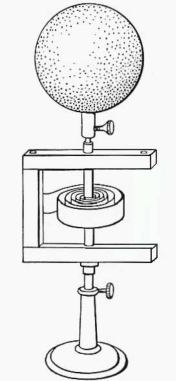
\includegraphics{Drillachse.pdf}
    \caption{Schematische Darstellung einer Drillachse\cite{ap05}.}
    \label{fig:drillachse}
\end{figure}
Optimalerweise sollte die Federwaage senkrecht zum Radius der Kreisbahn sein, da sich das in Gleichung \eqref{eq:drehmombetrag} beschriebene Drehmoment zu $M =F r$ vereinfacht.
Nun wird die Drillachse um zehn verschiedene Winkel ausgelenkt und jedes Mal wird die von der Federwaage gemessene Kraft aufgetragen. \\

Zur Bestimmung des Eigenträgheitsmoments $I_D$ werden zwei Gewichte im Abstand $a$ an der senkrecht zur Drehachse montierten Metallstange befestigt und das System wird um $\varphi = \dfrac{π}{2}$ ausgelenkt.
Es wird die dreifache Schwingungsdauer $3T$ gemessen und die Messung wird für zehn verschiedene Abstände $a$ wiederholt. \\

Anschließend werden die Schwingungsdauern einer Kugel und eines Zylinders analog ermittelt. Zusätzlich werden noch alle für die späteren Berechnungen der Theoriewerte notwendigen Körperparameter gemessen.
Dazu zählen das Gewicht, der Radius der Kugel sowie Höhe und Radius des Zylinders. \\

Diese Messung wird auch für eine Holzpuppe durchgeführt. Dabei werden die Längen und Durchmesser der einzelnen Körperteile, sprich Arme; Beine; Kopf und Torso, dokumentiert und es wird erneut die dreifache Schwingungsdauer
gemessen. Zur Messung der Durchmesser wird für jedes Körperteil an zehn unterschiedlichen Stellen gemessen und anschließend gemittelt. Die Schwingungsdauern werden bei zwei unterschiedlichen Körperhaltungen der Puppe aufgenommen.

Bei der erste Position stehen die Arme senkrecht vom Torso ab. Die Beine befinden sich parallel zur Rotationsachse. Kopf und Torso sind unbeweglich und befinden sich auf der Rotationsachse.
In der zweiten Position ist die Stellung der Arme unverändert und die Beine stehen ebenfalls senkrecht vom Körper ab. 


%%%%% korrigiert